\documentclass[a4paper,12pt]{article} 
\usepackage[utf8]{inputenc}
\usepackage{geometry}
\usepackage{listings}
\usepackage{xcolor}
\usepackage{hyperref}
\geometry{margin=1in}
\usepackage{graphicx}

\title{Controller Layer}
\date{\today}

\lstset{
  basicstyle=\ttfamily\small,
  keywordstyle=\color{blue}\bfseries,
  stringstyle=\color{red},
  commentstyle=\color{gray},
  breaklines=true,
  frame=single,
}

\begin{document}

\maketitle

\section{Understanding the Controller Layer and Integration Testing in Spring Boot}

\subsection{Introduction to the Controller Layer}
The \textit{Controller Layer} is a crucial part of a Spring Boot application. It handles HTTP requests from clients and maps them to appropriate services or business logic. By using controllers, we define the \textit{endpoints} of our REST API, enabling clients to perform operations like creating, reading, updating, or deleting resources.

\subsubsection{Role of the Controller Layer}
\begin{itemize}
    \item Acts as the \textit{gateway} to the application.
    \item Transforms client requests into appropriate service calls.
    \item Handles both incoming data (from request bodies) and outgoing responses (returned to the client).
    \item Ensures that the application adheres to the principles of RESTful architecture.
\end{itemize}

\subsubsection{Key Annotations in Controllers}
\begin{itemize}
    \item \texttt{@RestController}: Marks a class as a controller where every method returns a response body.
    \item \texttt{@RequestMapping}: Maps HTTP requests to specific methods or classes.
    \item \texttt{@PostMapping}, \texttt{@GetMapping}, \texttt{@PutMapping}, \texttt{@DeleteMapping}: Map HTTP methods (POST, GET, PUT, DELETE) to specific operations.
    \item \texttt{@RequestBody}: Binds the body of a client’s request to a method parameter.
    \item \texttt{@PathVariable}: Extracts a value from the URI for use in the method.
    \item \texttt{@Autowired}: Injects dependencies like services into the controller.
\end{itemize}
\noindent\begin{figure}[h!]
    \centering
    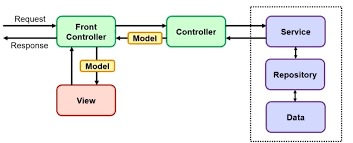
\includegraphics[width=\textwidth]{images/controller_layer01.jpg}
    \caption{Diagram of the Controller Layer interacting with other components such as Services, Repositories, and Clients.}
    \label{fig:controller_layer_diagram}
\end{figure}
\section{The Controllers We Built}
\subsection{Author Controller}
\textbf{Purpose}: Manages authors with details like \texttt{name} and \texttt{age}.
\begin{itemize}
    \item \textbf{Endpoints}:
    \begin{itemize}
        \item \textbf{Create}: \texttt{POST /api/authors/save} - Adds a new author to the system.
        \item \textbf{Read}:
        \begin{itemize}
            \item \texttt{GET /api/authors/all}: Retrieves all authors.
            \item \texttt{GET /api/authors/one/\{id\}}: Fetches a specific author by ID.
        \end{itemize}
        \item \textbf{Update}: \texttt{PUT /api/authors/update/\{id\}} - Modifies an author's details.
        \item \textbf{Delete}: \texttt{DELETE /api/authors/delete/\{id\}} - Removes an author by ID.
    \end{itemize}
\end{itemize}

\textbf{Example of Code: Author Controller}
The following example demonstrates the implementation of a controller layer (Author Controller as example).
It contains the annotations and all the features required for this layer.

The complete code is available on the project's GitHub repository: 
\hspace{5}\\

\url{https://github.com/D0esN0tM1tter/spring_boot_project-/blob/master/supporting_project/supporting_project/src/main/java/com/example/demo/controllers/AuthorController.java}.

\vspace{0.5cm}\\

\textbf{Explanation}:
\begin{itemize}
    \item The class is annotated with \texttt{@RestController}, indicating that it handles HTTP requests and provides responses in JSON format.
    \item The \texttt{@PostMapping("/save")} annotation specifies the endpoint for saving an author.
    \item \texttt{AuthorService} is injected using \texttt{@Autowired} to handle business logic.
    \item The \texttt{create()} method takes an \texttt{AuthorDto} object, calls the service layer to save it, and returns a response with status \texttt{201 CREATED}.
\end{itemize}
\subsection{Book Controller}
\textbf{Purpose}: Handles books with attributes like \texttt{title}, \texttt{author}, \texttt{category}, and \texttt{publish date}.
\begin{itemize}
    \item \textbf{Endpoints}:
    \begin{itemize}
        \item \textbf{Create}: \texttt{POST /api/books/save} - Adds a new book.
        \item \textbf{Read}:
        \begin{itemize}
            \item \texttt{GET /api/books/all}: Retrieves all books.
            \item \texttt{GET /api/books/one/\{id\}}: Fetches a specific book by ID.
        \end{itemize}
        \item \textbf{Update}: \texttt{PUT /api/books/update/\{id\}} - Updates book details.
        \item \textbf{Delete}: \texttt{DELETE /api/books/delete/\{id\}} - Deletes a book.
    \end{itemize}
\end{itemize}

\textbf{Example of Code: Book Controller Integration Test}

The following example demonstrates the implementation of one of the controller layer integration tests.
It contains the annotations and all the JUnit and Mockmvc logic required for this layer.

The complete code is available on the project's GitHub repository: 
\hspace{5}\\

\url{https://github.com/D0esN0tM1tter/spring_boot_project-/blob/master/supporting_project/supporting_project/src/test/java/com/example/demo/services/BookServicesIntegrationTests.java}.

\subsection{Category Controller}
\textbf{Purpose}: Manages categories, which classify books.
\begin{itemize}
    \item \textbf{Endpoints}:
    \begin{itemize}
        \item \textbf{Create}: \texttt{POST /api/category/save} - Adds a new category.
        \item \textbf{Read}:
        \begin{itemize}
            \item \texttt{GET /api/category/all}: Lists all categories.
            \item \texttt{GET /api/category/one/\{id\}}: Fetches a specific category by ID.
        \end{itemize}
        \item \textbf{Update}: \texttt{PUT /api/category/update/\{id\}} - Updates category details.
        \item \textbf{Delete}: \texttt{DELETE /api/category/delete/\{id\}} - Deletes a category.
    \end{itemize}
\end{itemize}

\section{Integration Testing: MockMvc and JSON-DTO-Entity Transformation}

\subsection{Why Testing is Important}
Testing helps verify that:
\begin{itemize}
    \item Each controller handles requests as expected.
    \item Data flows correctly between controllers and services.
    \item The system responds gracefully to errors or invalid inputs.
\end{itemize}
\subsection{Testing Options and Why We Chose MockMvc}

When developing a web application, several testing options are available. For instance, tests can be performed on the server side using technologies such as JPA, Thymeleaf, or by using frontend frameworks like Angular to test the interaction between the client and the server.

\subsection{Possible Approaches to Testing}
\begin{itemize}
    \item \textbf{Server-side Testing (JPA, Thymeleaf)}: 
    \begin{itemize}
        \item Server-side tests involve testing the business logic in the backend. For example, JPA (Java Persistence API) can be used to test interactions with the database, ensuring that entities are correctly persisted and retrieved. 
        \item Thymeleaf, integrated with Tomcat, can be used to test the server-side generation of views using dynamic HTML templates. These tests check that data is correctly injected into HTML pages before rendering.
    \end{itemize}
    
    \item \textbf{Testing with Front-End Frameworks (Angular)}: 
    \begin{itemize}
        \item Another type of test is to test the interactions between the frontend and backend. Frameworks like Angular allow simulating HTTP requests and verifying that the server responds correctly to user actions. These tests not only verify the integration of the frontend with the backend but also the user interface and interactions with the API.
    \end{itemize}
\end{itemize}

\subsection{Why We Chose MockMvc}
While other testing methods could be used to test the application end-to-end, we chose to use \texttt{MockMvc} for our integration tests. This approach offers several advantages, including:
\begin{itemize}
    \item \textbf{Simplified Backend Testing}: \texttt{MockMvc} allows us to simulate HTTP requests directly on the controller without requiring a real server like Tomcat. This lets us test the integration of the controller and service layers without the need for a full server setup or frontend client like Angular.
    \item \textbf{Business Logic Verification}: Using \texttt{MockMvc}, we can verify that the business logic, request routing, and data transformation (via DTOs, entities, etc.) work as expected, while avoiding the additional complexities involved with configuring a full web server or frontend framework.
    \item \textbf{Isolation and Focus on the API}: This method enables us to test only the API, isolating the backend without the need for a frontend client. This makes tests faster and more focused, ensuring that we concentrate on the essential server-side components.
\end{itemize}

In summary, while alternatives such as JPA, Thymeleaf, or tests with Angular exist to test interactions between different components, using \texttt{MockMvc} allows us to effectively test the backend in isolation and focus on backend logic, all while simplifying the testing process.

\subsection{Role of MockMvc}

\subsubsection{What is MockMvc?}
MockMvc is a Spring tool that allows us to test controllers without starting a server. It simulates HTTP requests and provides responses just like a real client-server interaction.
\subsubsection{2. Why MockMvc?}
\begin{itemize}
    \item Avoids the need for a running server.
    \item Mocks the HTTP request and response process.
    \item Ideal for integration testing since it ensures that the controller interacts correctly with the service layer and other components.
\end{itemize}

\subsubsection{3. Steps for Testing Using MockMvc:}
\begin{itemize}
    \item Configure MockMvc with \texttt{@AutoConfigureMockMvc} in your test class.
    \item Use MockMvc to simulate HTTP requests (e.g., POST, GET).
    \item Assert the expected status codes, headers, and response bodies.
\end{itemize}

\subsection{MockMvc Example: BookController Tests}
\subsubsection{1. Test for Creating a Book}
\textit{Simulates a POST request to create a new book. Converts a BookDto object to JSON, sends the JSON payload via MockMvc, and verifies the status code (201 Created) and response content (e.g., title, author).}

\newpage
\begin{lstlisting}[language=Java]
@Test
public void testCreateBook() throws Exception {
    AuthorDto author = new AuthorDto("Sami", 21);
    CategoryDto category = new CategoryDto("Info");
    BookDto book = new BookDto("Java", author, category, parseDate("2024-11-20"));

    String bookJson = objectMapper.writeValueAsString(book);

    mockMvc.perform(MockMvcRequestBuilders.post("/api/books/save")
            .contentType(MediaType.APPLICATION_JSON)
            .content(bookJson))
            .andExpect(MockMvcResultMatchers.status().isCreated())
            .andExpect(MockMvcResultMatchers.jsonPath("$.title").value("Java"))
            .andExpect(MockMvcResultMatchers.jsonPath("$.author.name").value("Sami"));
}
\end{lstlisting}
\subsubsection{ Test for Finding a Book by ID}
\begin{itemize}
    \item Simulates a GET request to fetch a book by ID.
    \item Verifies the response status (200 OK) and content (e.g., book title, author).
\end{itemize}

\subsubsection{ Test for Finding All Books}
\begin{itemize}
    \item Simulates a GET request to fetch all books.
    \item Verifies the list of books in the response.
\end{itemize}

\subsubsection{MockMvc Integration in Test Class}
\begin{itemize}
    \item \texttt{@SpringBootTest}: Loads the entire application context for testing.
    \item \texttt{@AutoConfigureMockMvc}: Enables MockMvc for integration tests.
    \item \texttt{MockMvc.perform}: Executes HTTP requests.
    \item \texttt{ObjectMapper}: Serializes Java objects to JSON and vice versa.
\end{itemize}

\subsection{3.3.2 Why Integration Tests?}
Integration tests validate the interaction between:
\begin{itemize}
    \item \textbf{Controller and Service layers}.
    \item \textbf{DTOs, Entities, and JSON}.
\end{itemize}
\section{Utility of JSON-DTO-Entity Transformation in a Layered Project}

\subsection{JSON-DTO-Entity Transformation}

In our layered project, the \textbf{JSON-DTO-Entity transformation} is a critical design pattern that ensures clean data flow between different application layers.

\begin{itemize}
    \item \textbf{JSON}:
    \begin{itemize}
        \item Represents the data exchanged between the client and the server.
        \item Used as the standard format for HTTP request and response bodies due to its simplicity and readability.
    \end{itemize}
    \item \textbf{DTO (Data Transfer Object)}:
    \begin{itemize}
        \item Acts as an intermediary between the client and the internal layers of the application.
        \item Enables validation and shaping of incoming and outgoing data without exposing the database structure.
        \item Prevents tight coupling between external APIs and internal domain models.
    \end{itemize}
    \item \textbf{Entity}:
    \begin{itemize}
        \item Represents the actual database structure used for persistence.
        \item The Service Layer converts DTOs into Entities for database operations and vice versa.
    \end{itemize}
\end{itemize}
\noindent\begin{figure}[h!]
    \centering
    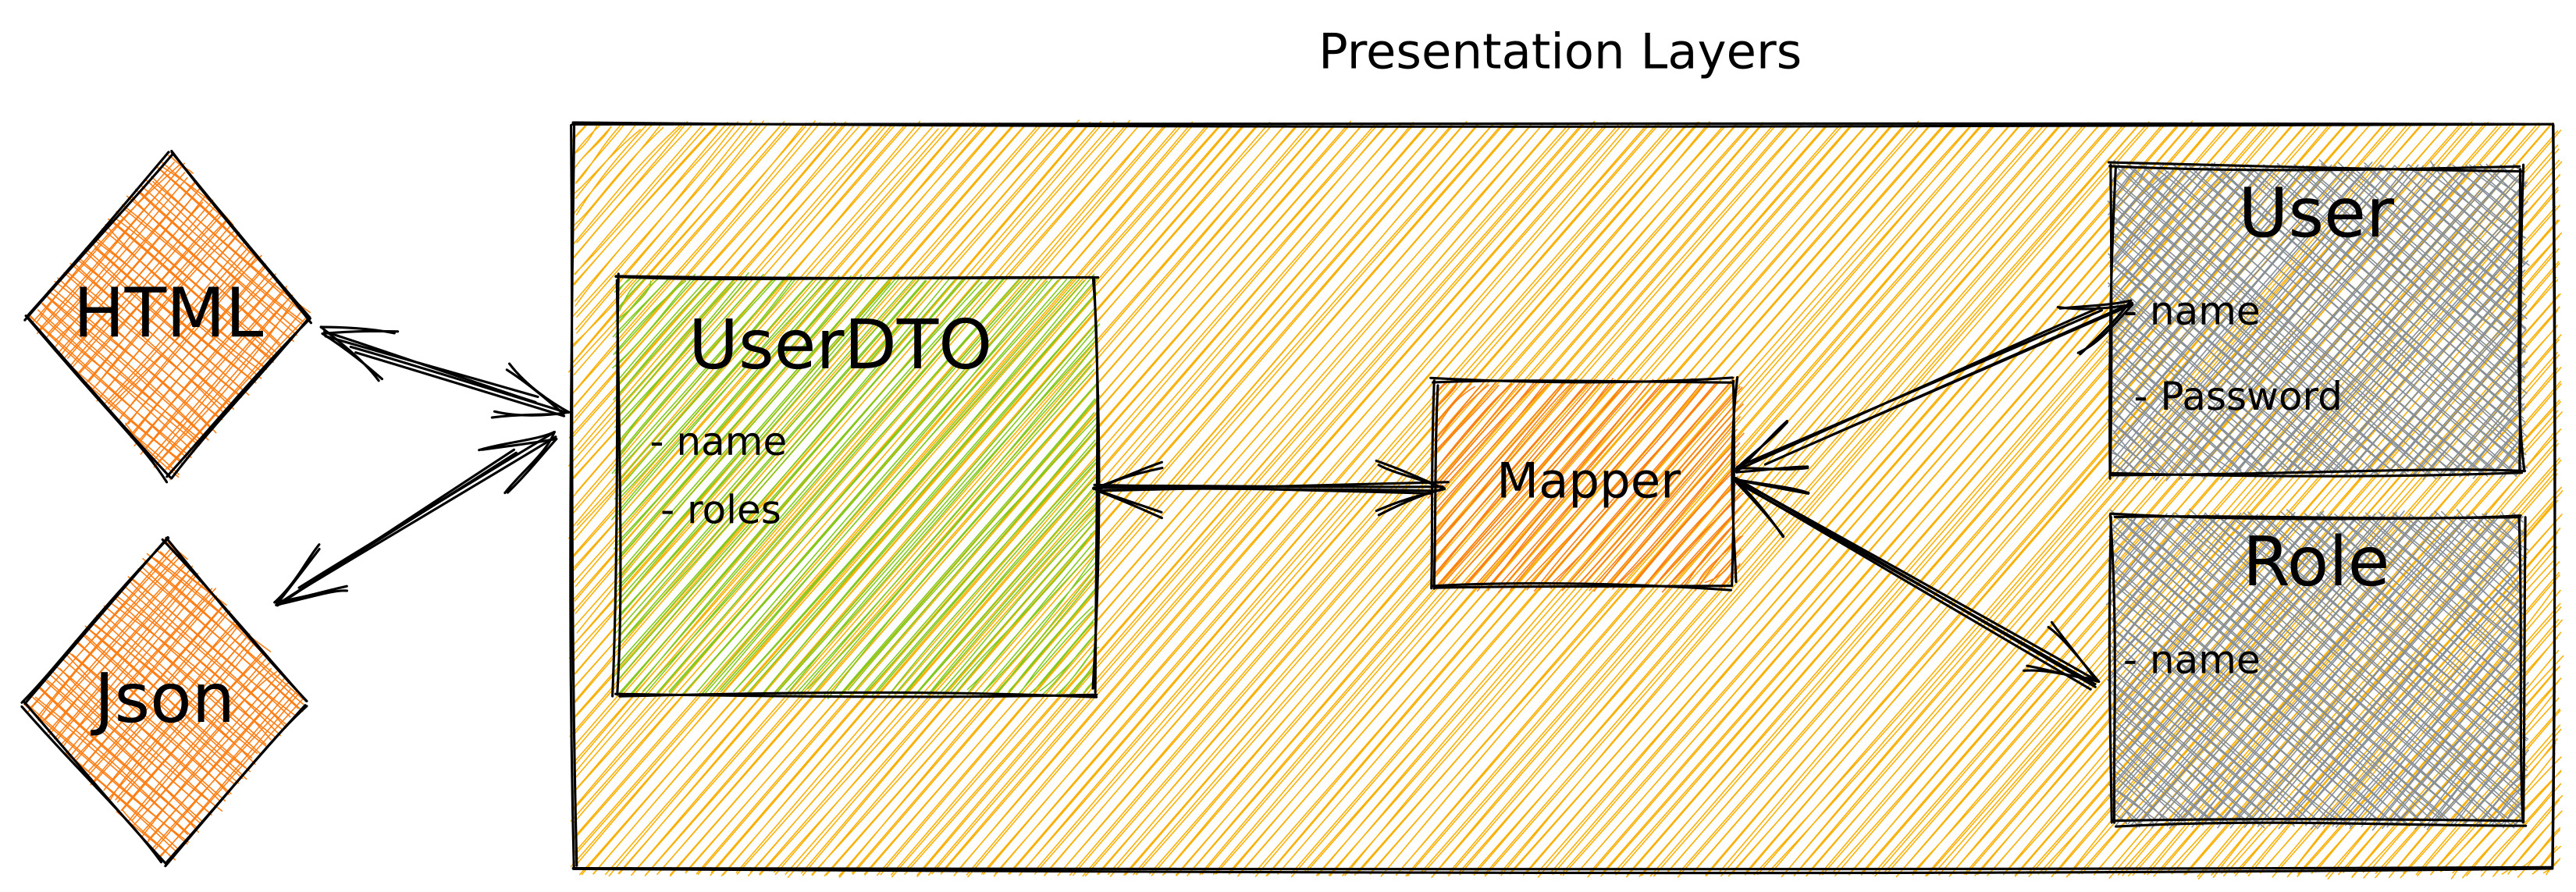
\includegraphics[width=\textwidth]{images/layers-4.jpg}
    \caption{Add a flowchart showing the transformation from JSON $\rightarrow$ DTO $\rightarrow$ Entity.}
    \label{fig:Transformation_JSON_DTO_Entity_diagram}
\end{figure}
\section{Understanding REST Architecture}

Representational State Transfer (REST) is an architectural style used for designing networked applications. REST is built around the principles of statelessness, resource-oriented interactions, and the use of standard HTTP methods.

RESTful applications expose their resources through Uniform Resource Identifiers (URIs) and allow interaction with these resources using HTTP verbs such as:
\begin{itemize}
    \item \textbf{GET}: Retrieve a resource or a list of resources.
    \item \textbf{POST}: Create a new resource.
    \item \textbf{PUT}: Update an existing resource.
    \item \textbf{DELETE}: Remove a resource.
\end{itemize}

A RESTful system communicates using a stateless protocol, typically HTTP, which ensures scalability and simplicity. The data is commonly exchanged in formats like JSON or XML, making it lightweight and compatible with various client types.

REST plays a significant role in the development of modern web applications by enabling flexible and efficient interactions between clients and servers.

\subsection{REST in the Project Context}

In this project, REST was chosen to design APIs that facilitate communication between the client and server. These APIs manage resources such as user data, tasks, or transactions, following the REST principles. By adopting REST, the application benefits from improved modularity, easier integration with third-party systems, and simplified client-server interactions.
\subsection{Testing RESTful APIs with MockMvc}

The RESTful APIs implemented in this project were tested using \texttt{MockMvc}, a framework provided by Spring for testing web applications. By leveraging \texttt{MockMvc}, we ensured that the APIs adhered to REST principles and returned the expected results for all HTTP methods.

The tests focused on:
\begin{itemize}
    \item Verifying correct implementation of HTTP methods (GET, POST, PUT, DELETE).
    \item Checking resource accessibility through URIs.
    \item Validating response formats (e.g., JSON) and HTTP status codes.
    \item Ensuring proper handling of edge cases, such as invalid inputs or unauthorized access.
\end{itemize}

This approach ensures the reliability and correctness of the RESTful APIs, which are integral to the application's architecture and functionality.


\section{Conclusion}
In this report, we explored the key aspects of the Controller Layer in a Spring Boot application, emphasizing its role in handling HTTP requests and serving as the entry point to the application’s business logic. By detailing the construction and purpose of various controllers, including the Author, Book, and Category controllers, we demonstrated the practical implementation of REST principles. 

The integration of annotations like \texttt{@RestController}, \texttt{@RequestMapping}, and \texttt{@Autowired} enables streamlined development and adherence to modern web standards. Additionally, the incorporation of DTOs ensures a clean separation between client requests and the application’s data model.

To validate the functionality of these controllers, we leveraged \texttt{MockMvc} for integration testing. This approach allowed us to test API endpoints effectively without the overhead of a full server setup, providing rapid feedback on the correctness of controller logic and its interactions with the service layer.

By combining robust design principles with effective testing strategies, this report highlights a structured methodology for building and validating RESTful APIs in Spring Boot. This knowledge lays a strong foundation for developing scalable and maintainable web applications while ensuring reliable performance through comprehensive testing.

\end{document}
